\documentclass{article}
\usepackage{natbib}
\usepackage{graphicx}
\usepackage{float}
\usepackage{listings}

\title{High-Performance Data Analysis on Janus using Apache Spark}
\author{Nick Vanderweit \\
        Ning Gao \\
        Anitha Ganesha \\
        Michael Kasper}

\begin{document}
\maketitle

\section{Introduction}
Over the past decade, there has been considerable interest in high-level
strategies for evaluating algorithms in parallel over large data sets.
Google's seminal MapReduce paper \citep{dean-mapreduce} describes such a
general strategy, which had already been in use at Google at the time of
publication, for building highly-scalable parallel applications out of small
serial functions. In general, phrasing data parallelism in terms of
higher-order functions on parallel data structures has proven fruitful
for many applications. In this paper, we evaluate Spark, a library
designed to address some of the shortcomings of MapReduce, on an existing
supercomputer.

In the MapReduce model, data is broken into \emph{splits} of a given size
before processing. These are stored on a distributed filesystem as key/value
pairs. The master node then distributes splits among the remaining workers.
Each of these workers runs a \emph{Map} on its split, computing for each
key/value pair $(k_1, v_1)$ another pair $(k_2, v_2)$. Each of these output
pairs is stored on the filesystem and the master is informed of their
locations. The master node proceeds by forwarding these intermediate pairs to the
\emph{Reduce} workers, which are responsible for combining the results for each
intermediate key.

A commonly-used example for this process is a distributed word count. First,
the input file (e.g. a large database dump containing posts on an Internet
forum) is broken into splits of a given size (say 64MB). The splits store
$(k, v)$ pairs such that each $v$ is a record (a post). The \emph{Map} task
is responsible for mapping each record to a set of $(\mbox{word}, \mbox{count})$
pairs, which are written to the filesystem.

The next step is for a \emph{Reduce} worker to sort these records by key
and then sum together the values for each given key, and write out
a set of (word, count) records where the keys are now unique.

This simple example has interesting implications for MapReduce in general.
We can see that \emph{Map} tasks are highly-parallel, but \emph{Reduce}
introduces a serial bottleneck. In cases like parallel word count, where the
\emph{Reduce} is associative and commutative (i.e. forms a commutative
semigroup over the set of values), there is an additional opportunity for
parallelism. As such, MapReduce provides an additional task, called a
\emph{Combiner}, which assumes this structure and can be used to distill
the intermediate $(k, v)$ pairs before a \emph{Reduce}.

We can also see from this example a significant limitation of MapReduce: each
intermediate $(k, v)$ set is written to the distributed filesystem.  As such,
in order for MapReduce to be efficient, the individual tasks must be very
large.

However, some algorithms are not well-described by a simple map-and-then-reduce
pattern, and require multiple iterations.  If each iteration is small, the
algorithm's performance will be bottlenecked by this file I/O. For these
problems, another approach is needed.

Spark was designed at the UC Berkeley AMPLab to address these concerns using a
more flexible abstraction for distributed data \citep{zaharia}. Rather than
assuming that all intermediate data is stored on a filesystem, Spark uses
\emph{Resilient Distributed Datasets}, or RDDs, to represent data that is
stored on disk, cached in memory, or possibly has not been computed yet at all
\citep{zaharia_rdd}.  It is primarily targeted toward Scala, a statically-typed
functional language for the Java Virtual Machine.

\section{Overview}
One of the key insights of Spark is that reducing the strictness of a
computation can offer large gains in performance. This lies at the heart
of the notion of RDDs: it is often more efficient to represent a \emph{recipe}
for a result than to represent the result itself, especially when the data sets
are arbitrarily large. Some programmers may be familiar with the related
notion of a \emph{thunk} in functional programming.

To demonstrate this idea, consider the following code snippet in a
functional language like ML:

\begin{lstlisting}[language=ML]
let rdd = ...
let mapped = map (fun x -> x * 2) rdd
let filtered = filter (fun x -> x mod 4 == 2) mapped
let sum = List.fold_left (fun x y -> x + y) 0 filtered
...
\end{lstlisting}

In the MapReduce model, there would be a strict filesystem write after each of
these lines.  Spark does not impose such a restriction, and allows the data to
persist in memory between operations. In fact, it even goes a step beyond this.
By default, RDDs are stored lazily as chains of computations that would
produce an output value. This has several advantages: for one, it is much
more practical to recover failed nodes with such a recipe in hand. Also,
storing computations as a lazy data structure permits certain optimizations.
For instance, the above example contains a \texttt{map} composed with a
\texttt{filter}. If this computation is expressed as a data structure,
the Spark environment can dynamically optimize it to:

\begin{lstlisting}[language=ML]
let rdd = ...
let filtered = filter (fun x -> (x * 2) mod 4 == 2) mapped
let sum = List.fold_left (fun x y -> x + y) 0 filtered
...
\end{lstlisting}

This kind of optimization is known as \emph{deforestation}, the elimination
of intermediate data structures, and is used to greatly improve data
locality \citep{wadler}.

\section{Evaluation}
We conducted our evaluation of the Spark framework on the University of
Colorado's Janus supercomputer.  Janus consists of 1,368 nodes, each containing
two six core Intel Xeon Westmere-EP chips at 2.8 GHz, for a total of 12 cores
per node.  Additionally, each core has 2 GB of 1333 MHz DDR RAM, for a total of
24 GB per node \citep{tufo}. In our research, we employed Spark version
0.8.0 along with Scala version 2.9.3. During our testing of the Spark framework,
we access input files from Janus' **lustre distributed file system**. % WHAT ELSE
Our aim was to assess the Spark on Janus and determine optimal configurations
to achieve the best performance.

\subsection{Testing}
Following the example from Google's first paper on MapReduce, the first test we
performed was a parallel grep \citep{dean-mapreduce}. Here an application would
scan through a large test file, looking for lines that matched a given regular
expression, finally returning the total number of matched lines. Two series of
test were run on two different files sizes. We first wanted to see how Spark
scales in an ideal setting, where the entire data set fits in memory. ***This
way we avoid the large performance hit Spark takes writing intermediate results
to disk***.  Given that each node has a total of 24 GB of RAM, we limited our
first problem size to 20GB. This allowed a single node to contain the entire
problem in memory, leaving some space for the OS and other supporting
processes. We executed this first test with 1 to 5 nodes. The second test we
performed was run with 5 to 50 nodes, each processing a 100GB file.

Ten trials were performed for each test, allows us to compute average
runtimes. To compute the speedup, Spark runtimes were compared to the UNIX grep
commands serial runtime on the same file. Finally, during our first test on the
20 GB file, we evaluated performance using a different number of workers per
node.  In Spark, a worker is an executor with it's own JVM which processes it's
own portion of the distributed data set. By default, a single worker is
employed on each node. For this test, we wanted to see if this was the ideal
setting on Janus.

% page rank
    % overview
    % ...

\subsection{Results}
In the first Grep test, we examined how Spark scales over a 20GB file using 1
to 5 nodes. Additionally, each trial was executed with a different number
workers per node. Figure \ref{fig:workNodeTime} shows the average runtimes as
the number of nodes increases. Each line in this graph represents a different
number of workers per node. We clearly can see from this graph that 6 and 12
workers per node yields significantly worse performance, while the results
produced by 1 to 3 workers is relatively equal.

    \begin{figure}[H]
        \centering
        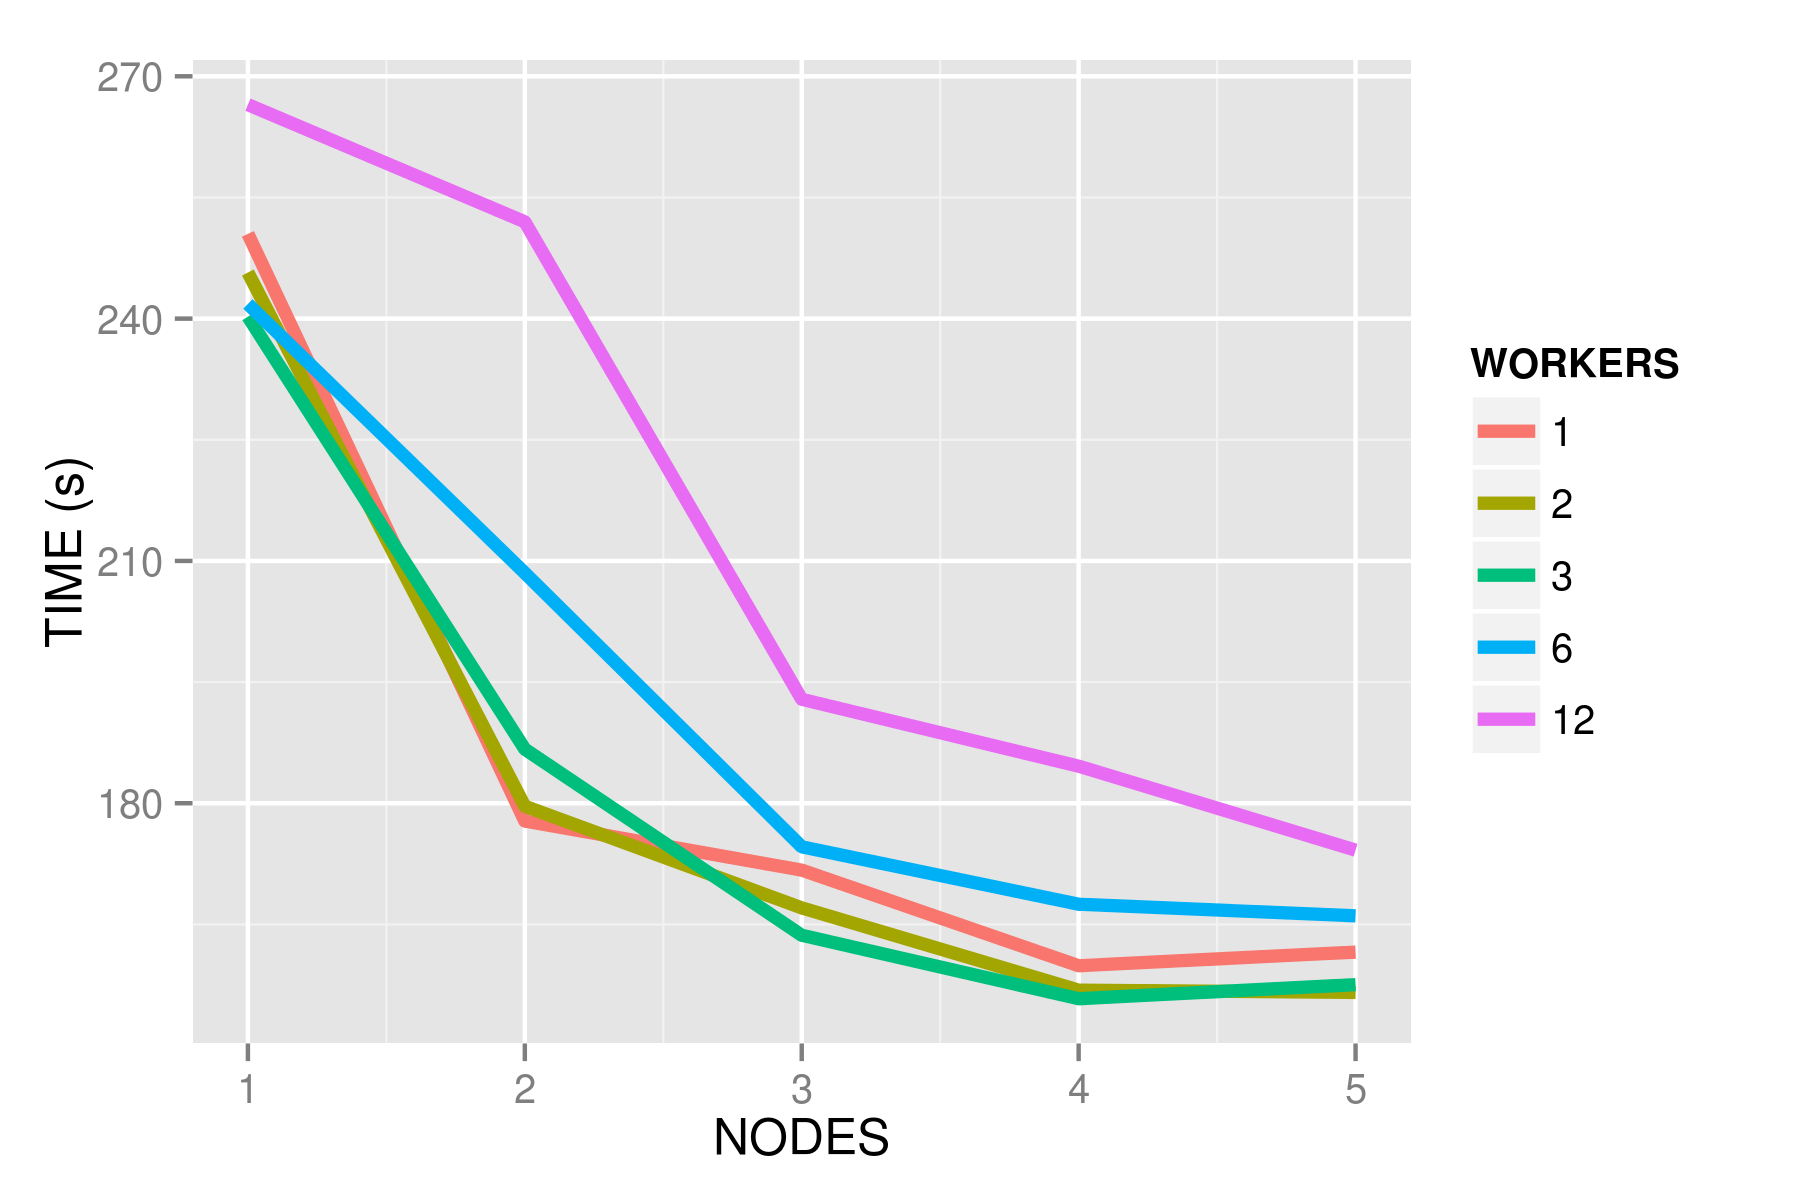
\includegraphics[width=90mm]{images/workerPerNodeTimes.png}
        \caption{Grep runtimes with different workers per node over 20GB file}
        \label{fig:workNodeTime}
    \end{figure}

Figure \ref{fig:workNodeSpeed} illustrates the results in terms of speedup.
Here we are comparing the resulting runtimes to the UNIX grep serial runtime of
1,120 seconds, processing the same 20 GB file. Note that here 1 node represents
12 cores.  So the initial speedup between 3 and 4 is not as impressive as one
might expect.  We also see that the speedup begins to level out around 4 nodes,
and in the case of 1 to 3 workers per node, it even decreases from 4 to 5
nodes.

    \begin{figure}[H]
        \centering
        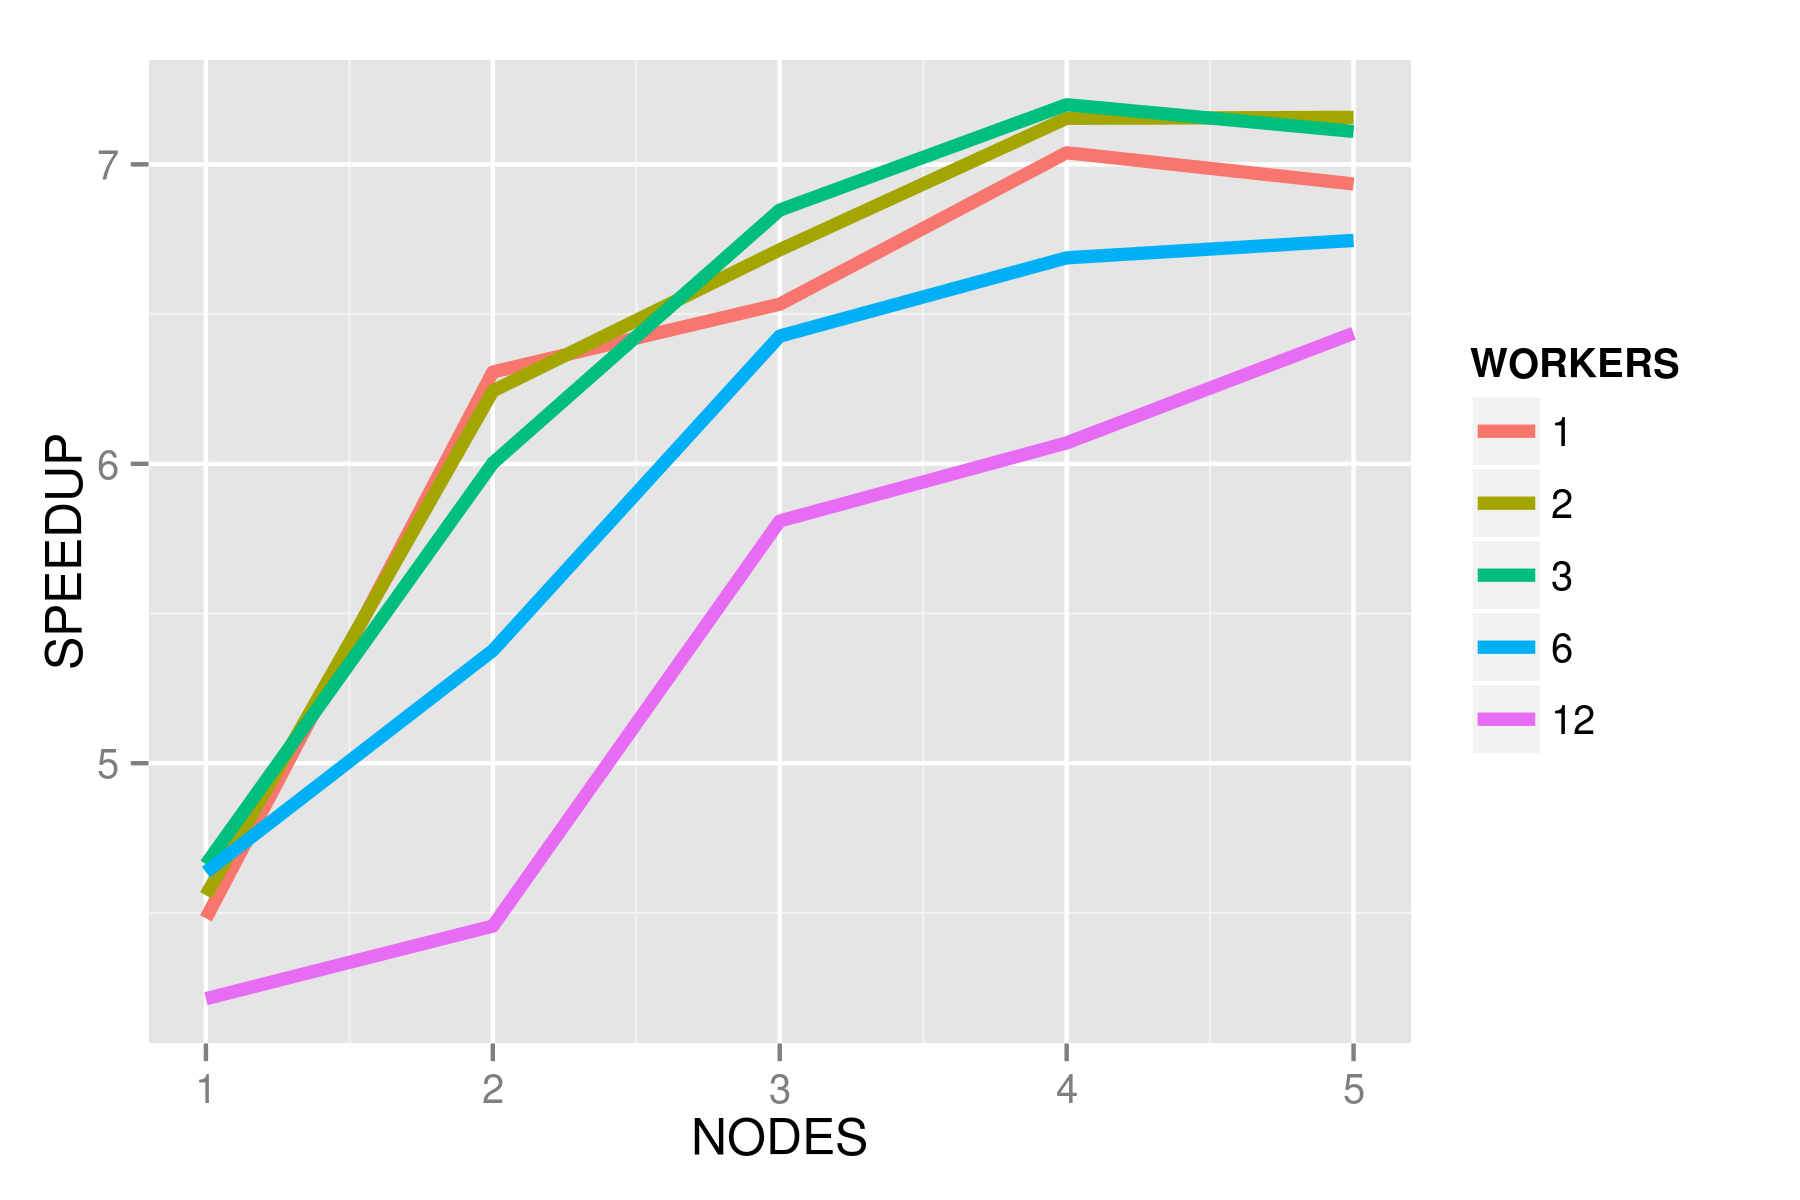
\includegraphics[width=90mm]{images/workerPerNodeSpeedup.png}
        \caption{Grep speedup with different workers per node over 20GB file}
        \label{fig:workNodeSpeed}
    \end{figure}

In the efficiency graph show in Figure \ref{fig:workNodeEff} we can see just
how well the cores are being utilized. As expected from the results shown in
the previous figures, the efficiency is quite poor. Employing a single node
starts just under 40\% efficiency. By the time we scale the problem to 5 nodes
(60 cores) we are just above 10\% efficiency.

    \begin{figure}[H]
        \centering
        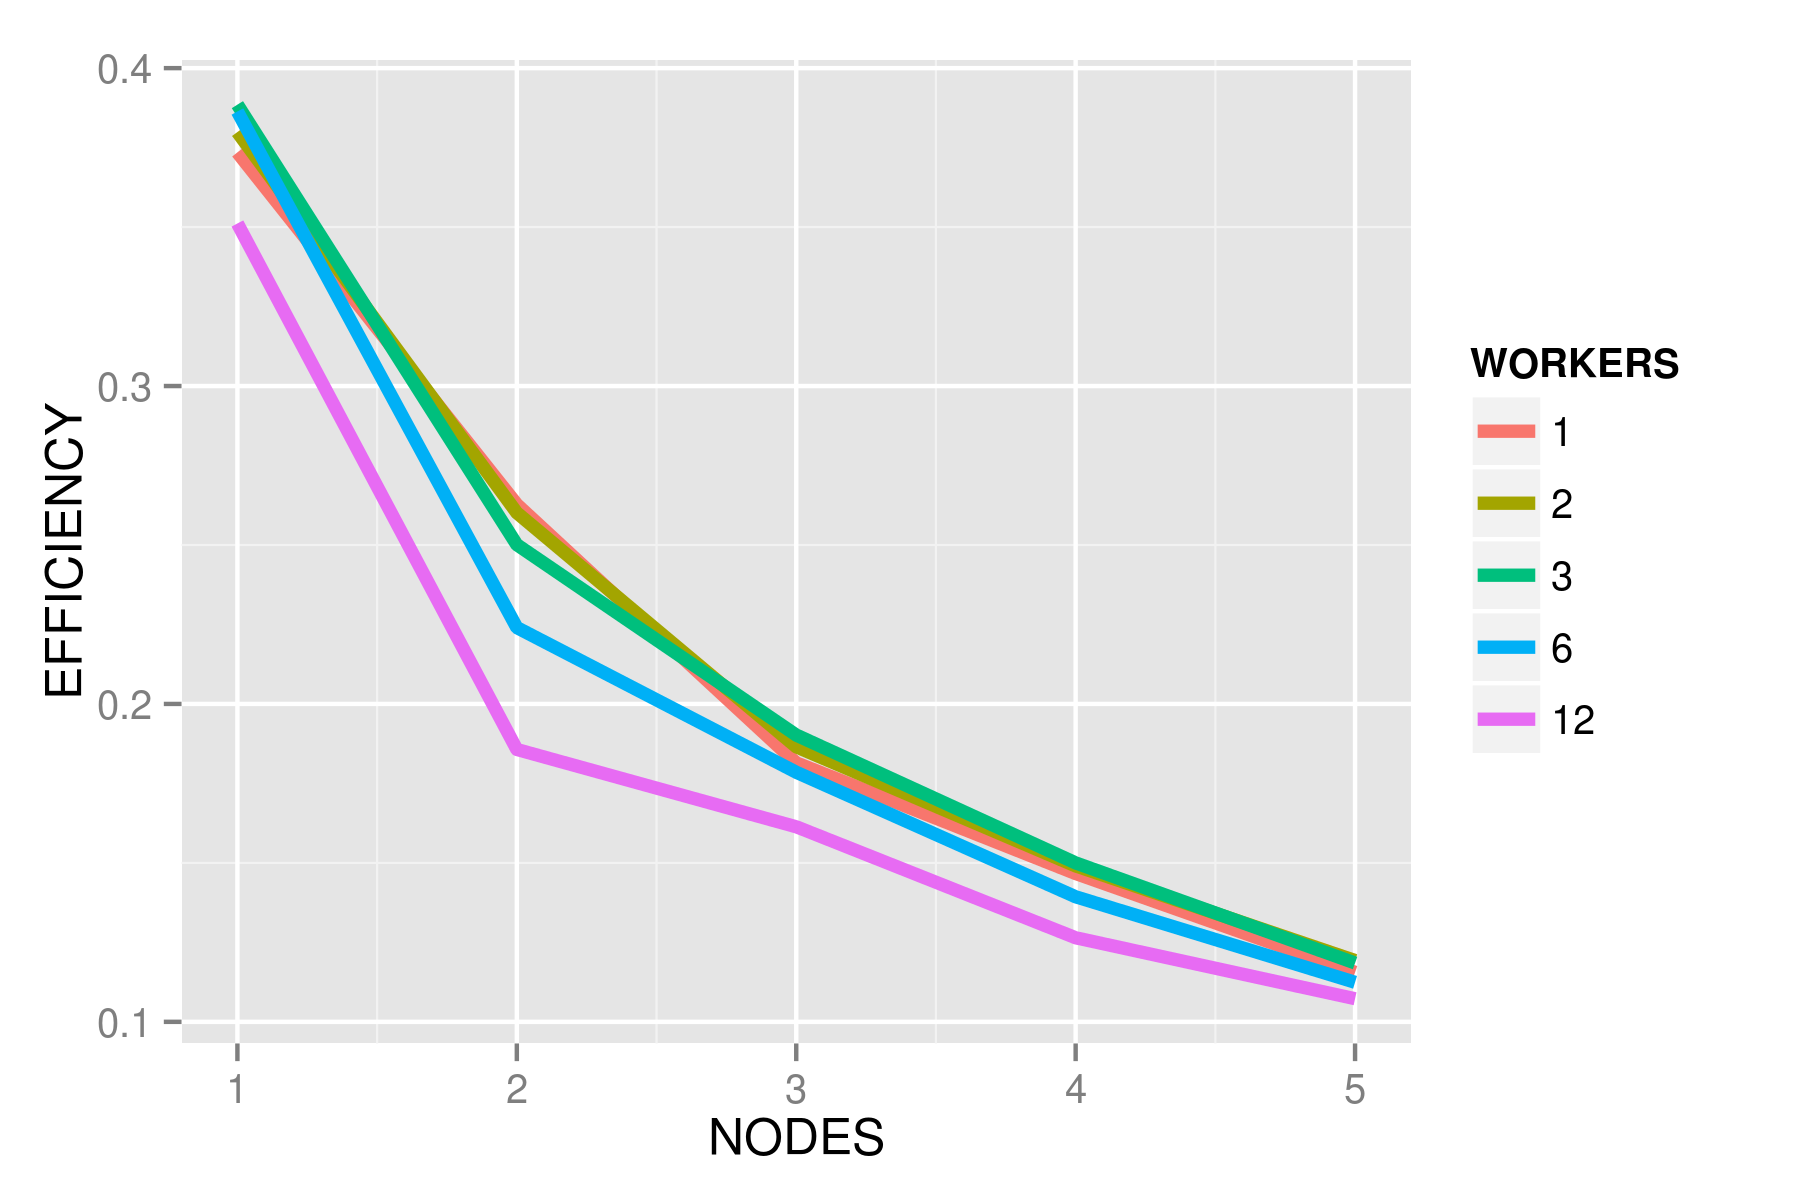
\includegraphics[width=90mm]{images/workerPerNodeEfficiency.png}
        \caption{Grep efficiency with different workers per node over 20GB file}
        \label{fig:workNodeEff}
    \end{figure}

Finally, Figure \ref{fig:workNodeKF} reflects the Karp-Flatt metric for the
runtime results. With the exception of the 12 workers per node (pink line), we
we see that the Karp-Flatt metric remains relatively constant, with values
between 0.12 and 0.14.  This constraint value would suggest that the large serial
portion of the application is what is preventing use from seeing better
scaling.

    \begin{figure}[H]
        \centering
        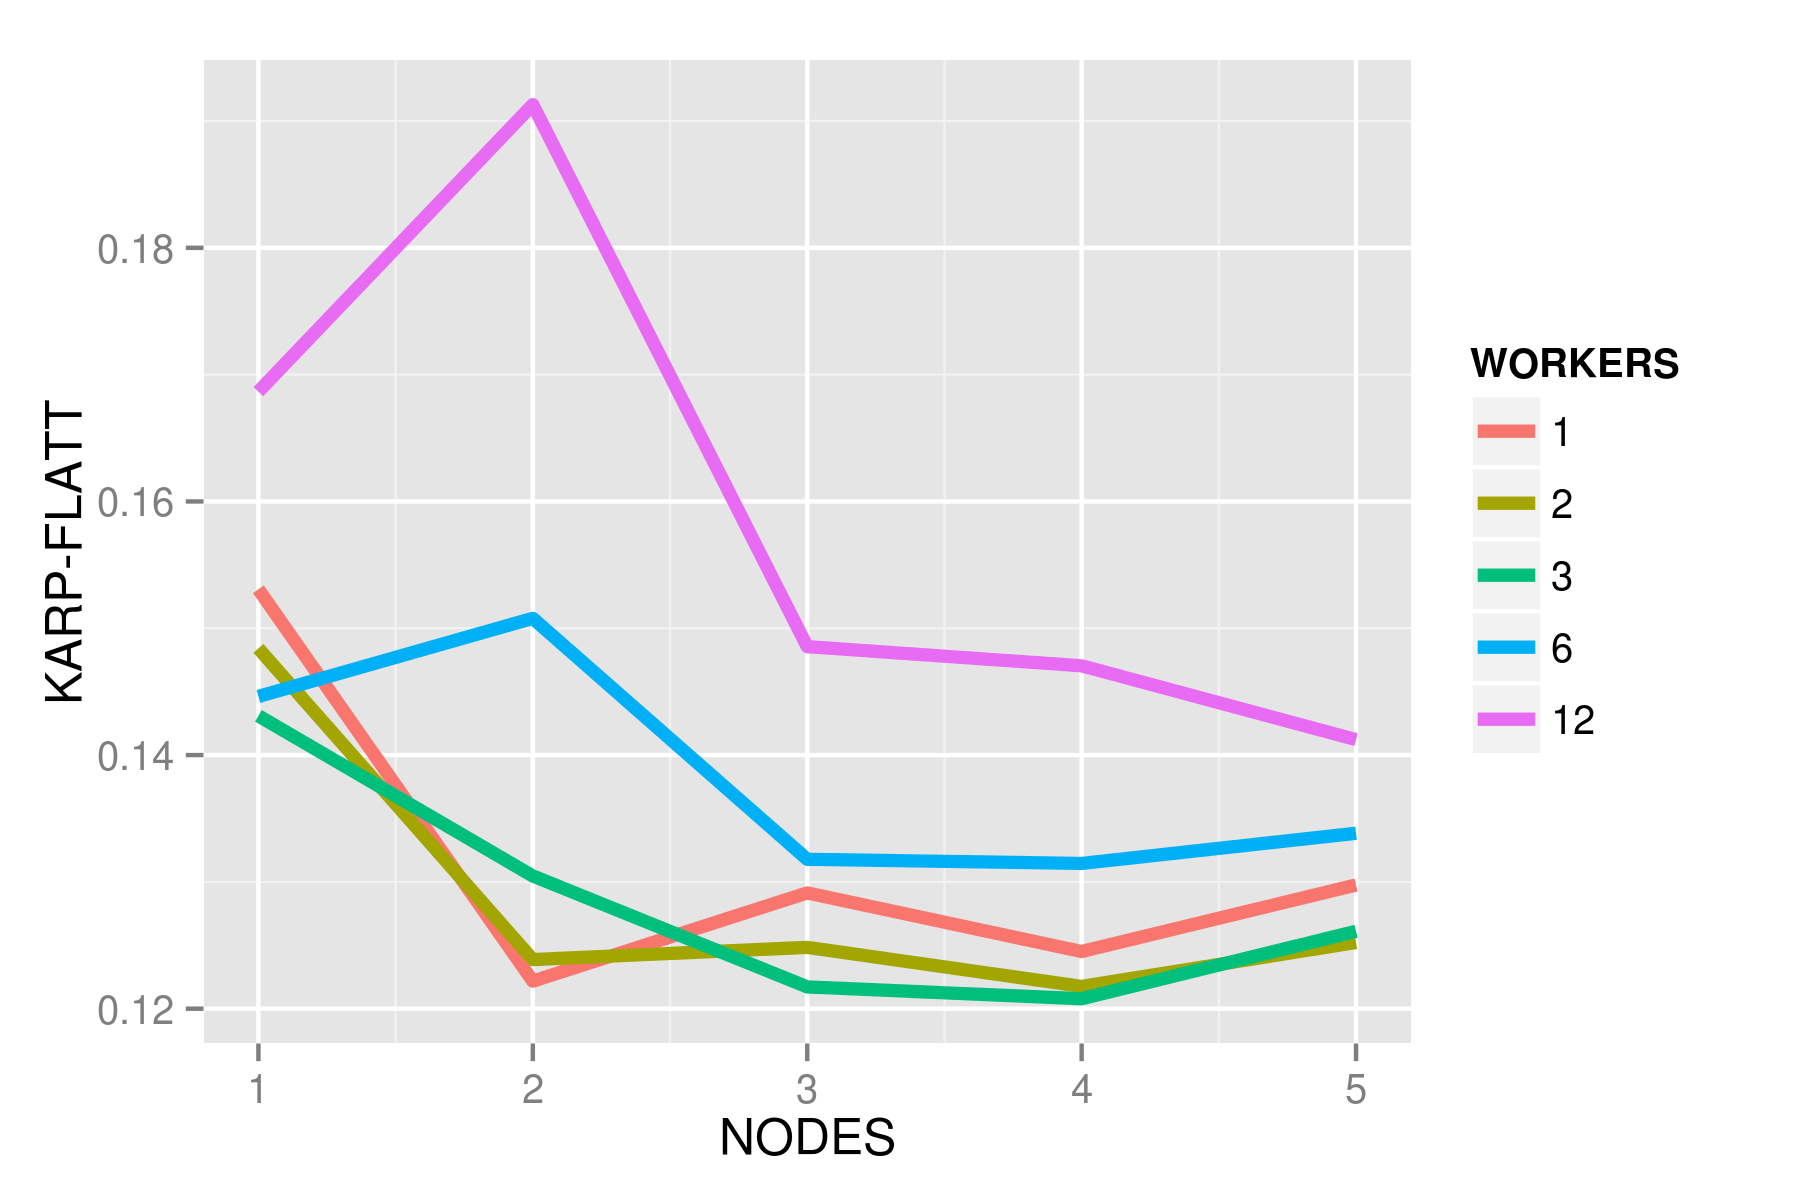
\includegraphics[width=90mm]{images/workerPerNodeKarpFlatt.png}
        \caption{Grep Karp-Flatt with different workers per node over 20GB file}
        \label{fig:workNodeKF}
    \end{figure}

To see if we could observe better scaling, we ran the same grep test over a
100 GB file.  During this test, we also increased the number of nodes used,
starting with 5 and going to 50 nodes. Given its size, the input text file was
accessed from the Janus' lustre filesystem. Figure \ref{fig:bigTime} shows the
runtimes observed over this large problem.  Clearly there appears to be no
change in runtimes, as the runtimes hover around 500 seconds, regardless of the
number of nodes used. Suspecting the short computational time of the grep
search, we began running our tests on the more computationally expensive
PageRank algorithm.

    \begin{figure}[H]
        \centering
        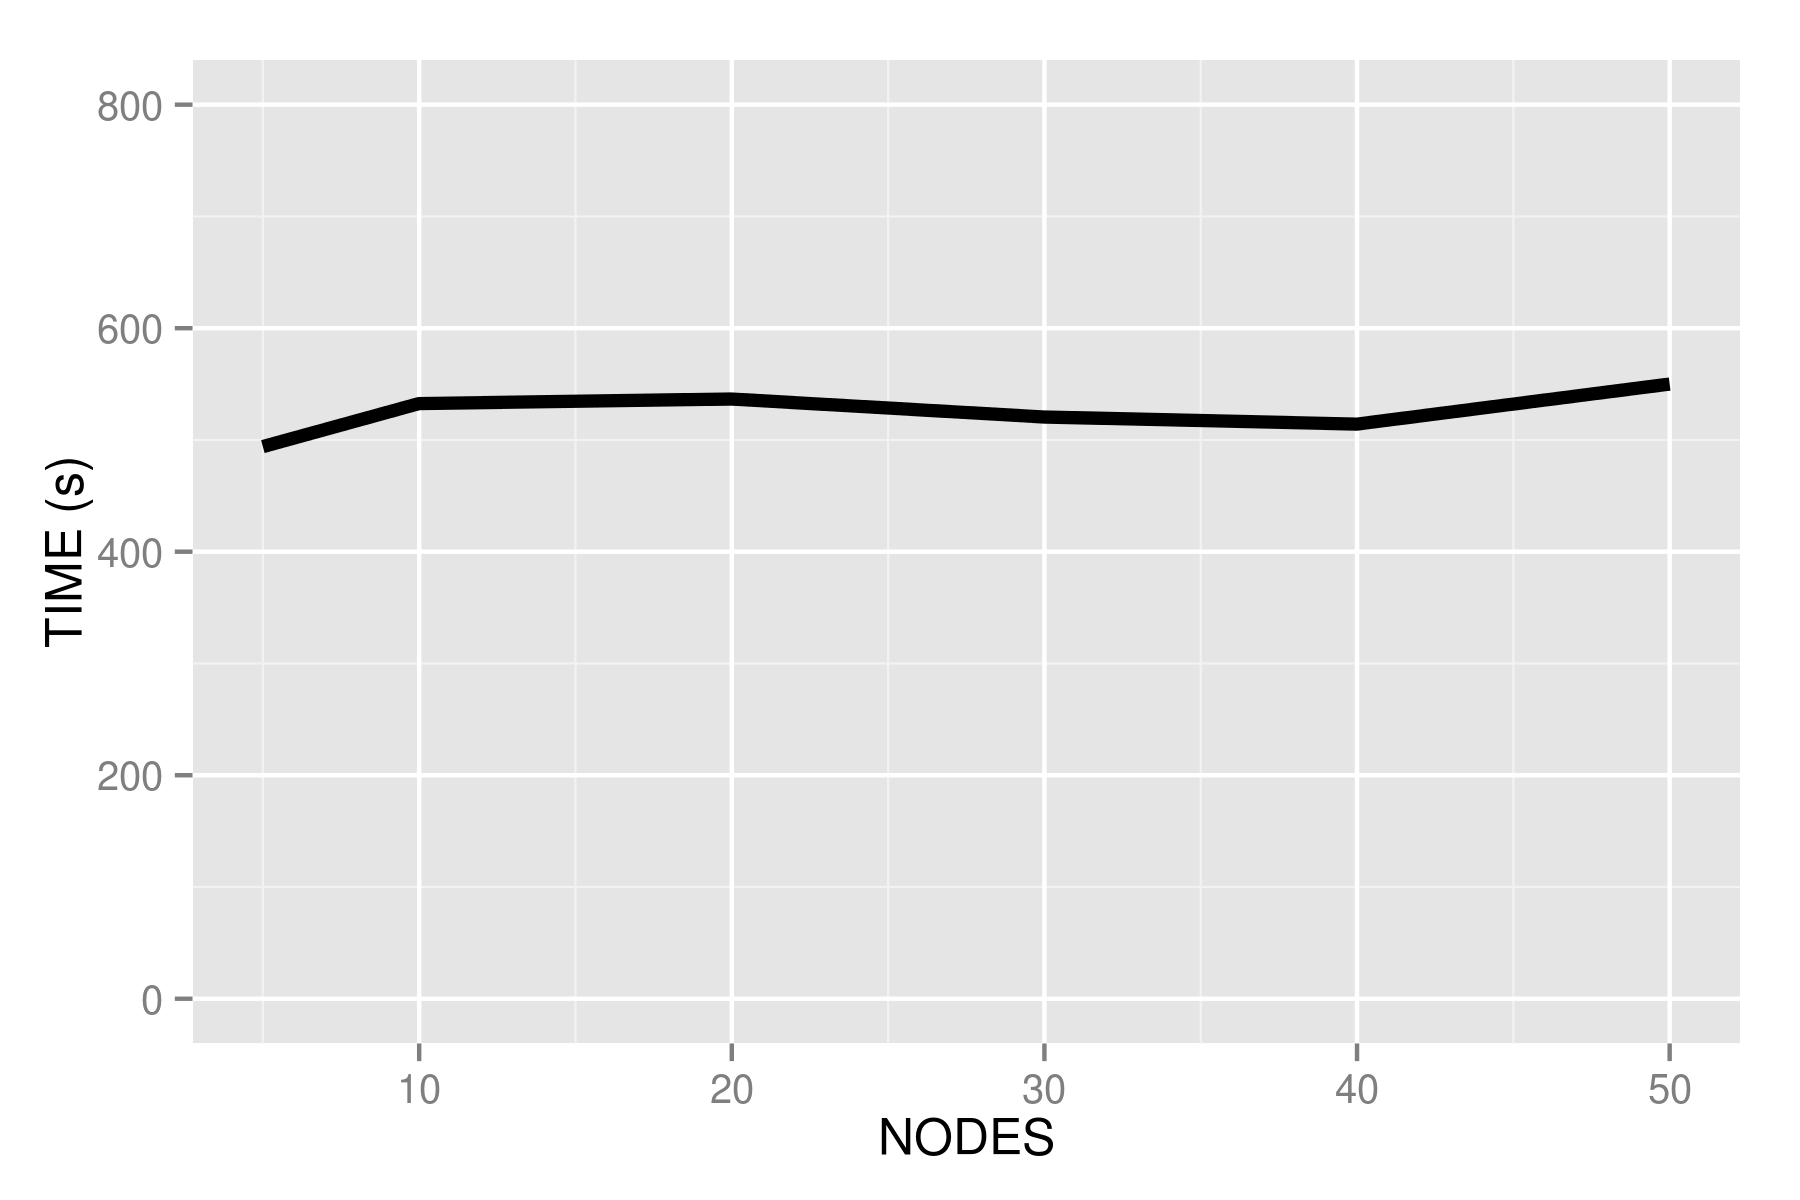
\includegraphics[width=90mm]{images/bigDataTimes.png}
        \caption{Average grep runtimes over 100GB file}
        \label{fig:bigTime}
    \end{figure}

% pagerank test 1
% pagerank test 2
% ...

\section{Discussion}
The results collected from the initial grep test over the 20 GB file gave us
some insight on how well such a problem scales in the Spark framework.  Given
that text file of 20 GB, it appears that employing 3 nodes provides a good
balance between speedup and efficiency.  We also saw how the number of workers
per node effects the overall runtime. While 1 to 3 workers yield relatively
similar results, it seems that using 2 to 3 nodes may give a slight performance
increase. This test would need to be run several more times to achieve more
more conclusive runtime averages.  It would also be beneficial to increase the
input file size and node codes, to see if the observed trend continues as the
problem scales.

In the grep test over the 100 GB file, surprisingly we observed practically no
change in runtime performance. Perhaps the Karp-Flatt metric results in the
previous test gives us some insight as to why this is the case. We suspect the
long load times on this larger file greatly outweigh any speedup achieved
through running grep on multiple workers. Given that, we also suspect that
Spark could be reading this file in serial from the lustre file system. The
lack of Spark logging and profiling tools makes it difficult to determine
exactly how long each stage is takes. But further investigation would be needed
to determine a possible solution or workaround.

% pagerank test 1
% pagerank test 2
% ...

% other problems exhibited
    % easy to install, hard to configure/profile/understand results
    % sporadic runtimes 

% workers and master communication over spark protocol

\section{Conclusion}

\bibliography{paper}
\bibliographystyle{plain}

\end{document}
